\documentclass{article}

% content/resources/templates/preamble.tex
\usepackage[margin=0.6in]{geometry}
\author{Milav Dabgar}
\usepackage{amsmath,amssymb,amsthm}
\usepackage{booktabs}
\usepackage{multirow}
\usepackage{xcolor}
\usepackage{tcolorbox}
\tcbuselibrary{breakable,skins}
\usepackage[colorlinks=true,linkcolor=blue]{hyperref}
\usepackage{titlesec}
\usepackage{enumitem}
\usepackage{tikz}
\usepackage{pgfplots}
\usepackage{circuitikz}
\usepackage[version=4]{mhchem}
\usepackage{longtable}
\usepackage{array}
\usepackage{float}
\usepackage{caption}
\usepackage{listings}

\lstset{
  basicstyle=\small\ttfamily,
  breaklines=true,
  breakatwhitespace=false,
  postbreak=\mbox{\textcolor{red}{$\hookrightarrow$}\space},
  float=false,
  numbers=left,
  numberstyle=\tiny\color{gray},
  numbersep=10pt,
  xleftmargin=2em,
  keywordstyle=\color{blue},
  commentstyle=\color{green!60!black},
  stringstyle=\color{purple},
  backgroundcolor=\color{gray!5},
  showstringspaces=false,
  tabsize=2,
  captionpos=b,
  keepspaces=true,
  columns=flexible
}

\pgfplotsset{compat=1.18}
\usetikzlibrary{shapes,arrows,positioning,calc,patterns,decorations.pathmorphing,decorations.markings,arrows.meta}

% Color scheme
\definecolor{headcolor}{RGB}{0,102,204}
\definecolor{keycolor}{RGB}{220,20,60}
\definecolor{solutioncolor}{RGB}{34,139,34}
\definecolor{mnemoniccolor}{RGB}{148,0,211}
\definecolor{codecolor}{RGB}{0,0,100}

% Spacing
\setlength{\parskip}{3pt}
\setlist[itemize]{nosep}
\setlist[enumerate]{nosep}

% Title formatting
\titleformat{\section}{\Large\bfseries\color{headcolor}}{\thesection}{1em}{}
\titleformat{\subsection}{\large\bfseries\color{headcolor}}{\thesubsection}{1em}{}

% Pandoc tightlist compatibility
\providecommand{\tightlist}{%
  \setlength{\itemsep}{0pt}\setlength{\parskip}{0pt}}

% Pandoc longtable compatibility
\newcounter{none}
\def\thenone{}


% content/resources/templates/english-boxes.tex

% Custom environments
\newtcolorbox{solutionbox}{
 breakable,
 enhanced,
 colback=solutioncolor!5!white,
 colframe=solutioncolor!75!black,
 fonttitle=\bfseries,
 title=Solution
}

\newtcolorbox{solutionboxnobreak}{
 colback=solutioncolor!5!white,
 colframe=solutioncolor!75!black,
 fonttitle=\bfseries,
 title=Solution
}

\newtcolorbox{keyformula}{
 breakable,
 enhanced,
 colback=keycolor!5!white,
 colframe=keycolor!75!black,
 fonttitle=\bfseries,
 title=Key Formula
}

\newtcolorbox{mnemonicboxenv}{
 breakable,
 enhanced,
 colback=mnemoniccolor!5!white,
 colframe=mnemoniccolor!75!black,
 fonttitle=\bfseries,
 title=Mnemonic
}

\newcommand{\mnemonicbox}[1]{%
  \begin{mnemonicboxenv}
    #1
  \end{mnemonicboxenv}
}


% Custom commands for GTU solutions
% This file defines semantic commands for consistent formatting

% Question command with automatic formatting
\newcommand{\question}[2]{%
  \section*{Question #1}%
  \textbf{#2}%
}

% OR question variant
\newcommand{\questionor}[2]{%
  \section*{Question #1 OR}%
  \textbf{#2}%
}

% Proper table environment with caption
\newenvironment{answertable}[1]{%
  \begin{table}[htbp]
  \centering
  \caption{#1}
}{%
  \end{table}
}

% Proper figure environment for diagrams
\newenvironment{answerdiagram}[1]{%
  \begin{figure}[htbp]
  \centering
  \caption{#1}
}{%
  \end{figure}
}

% Semantic markup for key terms
\newcommand{\keyword}[1]{\textbf{#1}}
\newcommand{\code}[1]{\texttt{#1}}
\newcommand{\classname}[1]{\texttt{#1}}
\newcommand{\methodname}[1]{\texttt{#1}}

% Proper quotation marks
\newcommand{\mnemonic}[1]{``#1''}


\title{Principles of Electronic Communication (4331104) - Summer 2024 Solution}
\date{June 14, 2024}

\begin{document}
\maketitle

\questionmarks{1}{a}{3}
\textbf{Draw and explain block diagram of communication system.}

\begin{solutionbox}
    \textbf{Answer}:

    \begin{center}
    \begin{tikzpicture}[auto, node distance=2.5cm, >=latex]
        \node [gtu block] (source) {Information Source};
        \node [gtu block, right of=source, node distance=3.5cm] (tx) {Transmitter};
        \node [gtu block, right of=tx, node distance=3.5cm] (channel) {Channel/Medium};
        \node [gtu block, right of=channel, node distance=3.5cm] (rx) {Receiver};
        \node [gtu block, right of=rx, node distance=3.5cm] (dest) {Destination};
        \node [gtu block, below of=channel, node distance=2cm] (noise) {Noise Source};

        \draw [gtu arrow] (source) -- (tx);
        \draw [gtu arrow] (tx) -- (channel);
        \draw [gtu arrow] (channel) -- (rx);
        \draw [gtu arrow] (rx) -- (dest);
        \draw [gtu arrow] (noise) -- (channel);
    \end{tikzpicture}
    \end{center}

    \begin{itemize}
        \item \textbf{Information Source}: Generates message signal (voice, video, data).
        \item \textbf{Transmitter}: Converts message to suitable form for transmission.
        \item \textbf{Channel}: Medium through which signal travels (wires, fiber, air).
        \item \textbf{Receiver}: Extracts original message from received signal.
        \item \textbf{Destination}: End-user who receives the information.
    \end{itemize}

    \begin{mnemonicbox}
    "Information Travels Carefully Reaching Destination"
    \end{mnemonicbox}
\end{solutionbox}

\questionmarks{1}{b}{4}
\textbf{Explain applications of EM wave spectrum.}

\begin{solutionbox}
    \textbf{Answer}:

    \begin{tabulary}{\textwidth}{|L|L|L|}
    \hline
    \textbf{Frequency Band} & \textbf{Frequency Range} & \textbf{Applications} \\
    \hline
    Radio waves & 3 kHz - 300 MHz & AM/FM broadcasting, maritime communication \\
    \hline
    Microwaves & 300 MHz - 300 GHz & Radar, satellite communication, microwave ovens \\
    \hline
    Infrared & 300 GHz - 400 THz & Remote controls, thermal imaging, optical fibers \\
    \hline
    Visible light & 400 THz - 800 THz & Fiber optic communication, photography \\
    \hline
    Ultraviolet & 800 THz - 30 PHz & Sterilization, authentication, water purification \\
    \hline
    X-rays & 30 PHz - 30 EHz & Medical imaging, security scanning, material analysis \\
    \hline
    Gamma rays & >30 EHz & Cancer treatment, food sterilization, industrial inspection \\
    \hline
    \end{tabulary}

    \begin{mnemonicbox}
    "Radio Makes Invisible Very eXtreme Gamma signals"
    \end{mnemonicbox}
\end{solutionbox}

\questionmarks{1}{c}{7}
\textbf{State and explain external and internal noise.}

\begin{solutionbox}
    \textbf{Answer}:

    \begin{tabulary}{\textwidth}{|L|L|L|}
    \hline
    \textbf{Type} & \textbf{External Noise} & \textbf{Internal Noise} \\
    \hline
    \textbf{Source} & Outside the communication system & Inside electronic components \\
    \hline
    \textbf{Types} & Atmospheric, Space, Industrial, Man-made & Thermal, Shot, Transit-time, Flicker \\
    \hline
    \textbf{Control} & Can be reduced by shielding, filtering & Reduced by better components, cooling \\
    \hline
    \textbf{Examples} & Lightning, Solar radiation, Motor sparking & Electron movement in resistors, semiconductors \\
    \hline
    \textbf{Nature} & Usually unpredictable, varying & More consistent and quantifiable \\
    \hline
    \end{tabulary}

    \textbf{Diagram:}

    \begin{center}
    \begin{tikzpicture}[gtu tree]
    \node [gtu block] {Noise in Communication}
        child {node [gtu block] {External Noise}
            child {node [gtu state] {Atmospheric\\Noise}}
            child {node [gtu state] {Space\\Noise}}
            child {node [gtu state] {Industrial\\Noise}}
            child {node [gtu state] {Man-made\\Noise}}
        }
        child {node [gtu block] {Internal Noise}
            child {node [gtu state] {Thermal\\Noise}}
            child {node [gtu state] {Shot\\Noise}}
            child {node [gtu state] {Transit-time\\Noise}}
            child {node [gtu state] {Flicker\\Noise}}
        };
    \end{tikzpicture}
    \end{center}

    \begin{mnemonicbox}
    "External Environmental Sources Invade; Internal Components Generate Noise"
    \end{mnemonicbox}
\end{solutionbox}

\questionmarks{1}{c}{7}
\textbf{Draw and explain the block diagram of a Superheterodyne AM receiver.}

\begin{solutionbox}
    \textbf{Answer}:

    \begin{center}
    \begin{tikzpicture}[auto, node distance=2cm, >=latex]
        % Nodes
        \node [gtu block] (rf) {RF Amplifier};
        \node [left of=rf, node distance=2.5cm] (ant) {Antenna};
        \node [gtu block, right of=rf, node distance=3cm] (mixer) {Mixer};
        \node [gtu block, below of=mixer, node distance=2cm] (lo) {Local Oscillator};
        \node [gtu block, right of=mixer, node distance=3cm] (if) {IF Amplifier};
        \node [gtu block, right of=if, node distance=3cm] (det) {Detector};
        \node [gtu block, right of=det, node distance=3cm] (af) {AF Amplifier};
        \node [right of=af, node distance=2.5cm] (spk) {Speaker};
        \node [gtu block, below of=if, node distance=2.5cm] (agc) {AGC};

        % Connections
        \draw [gtu arrow] (ant) -- (rf);
        \draw [gtu arrow] (rf) -- (mixer);
        \draw [gtu arrow] (lo) -- (mixer);
        \draw [gtu arrow] (mixer) -- (if);
        \draw [gtu arrow] (if) -- (det);
        \draw [gtu arrow] (det) -- (af);
        \draw [gtu arrow] (af) -- (spk);
        
        % AGC paths
        \draw [gtu arrow] (det.south) |- (agc.east);
        \draw [gtu arrow] (agc.west) -| (rf.south);
        \draw [gtu arrow] (agc.north) -- (if.south);

    \end{tikzpicture}
    \end{center}

    \begin{tabulary}{\textwidth}{|L|L|}
    \hline
    \textbf{Block} & \textbf{Function} \\
    \hline
    \textbf{RF Amplifier} & Amplifies weak radio signals and provides selectivity \\
    \hline
    \textbf{Local Oscillator} & Generates frequency for mixing with incoming signal \\
    \hline
    \textbf{Mixer} & Combines RF and local oscillator signals to produce IF \\
    \hline
    \textbf{IF Amplifier} & Amplifies signal at fixed intermediate frequency (455 kHz) \\
    \hline
    \textbf{Detector} & Extracts audio from modulated carrier (demodulation) \\
    \hline
    \textbf{AF Amplifier} & Amplifies audio signal to drive speaker \\
    \hline
    \textbf{AGC} & Automatic Gain Control - maintains constant output level \\
    \hline
    \end{tabulary}

    \begin{mnemonicbox}
    "Radio Loves Making Interesting Detected Audio Sounds"
    \end{mnemonicbox}
\end{solutionbox}

\questionmarks{2}{a}{3}
\textbf{Define modulation. State types of modulation.}

\begin{solutionbox}
    \textbf{Answer}:

    \textbf{Modulation}: Process of varying one or more properties of a high-frequency carrier signal with a modulating signal containing information.

    \textbf{Types of Modulation:}

    \begin{center}
    \begin{tikzpicture}[gtu tree, level distance=1.5cm, sibling distance=2cm]
    \node [gtu block] {Modulation}
        child {node [gtu block, align=center] {Analog\\Modulation}
            child {node [gtu state] {AM}}
            child {node [gtu state] {FM}}
            child {node [gtu state] {PM}}
        }
        child {node [gtu block, align=center] {Digital\\Modulation}
            child {node [gtu state] {ASK}}
            child {node [gtu state] {FSK}}
            child {node [gtu state] {PSK}}
        }
        child {node [gtu block, align=center] {Pulse\\Modulation}
            child {node [gtu state] {PAM}}
            child {node [gtu state] {PWM}}
            child {node [gtu state] {PPM}}
            child {node [gtu state] {PCM}}
        };
    \end{tikzpicture}
    \end{center}

    \begin{mnemonicbox}
    "All Modulations Alter Properties: Frequency, Amplitude, Phase"
    \end{mnemonicbox}
\end{solutionbox}

\questionmarks{2}{b}{4}
\textbf{Define: Signal to noise ratio and Noise figure.}

\begin{solutionbox}
    \textbf{Answer}:

    \begin{tabulary}{\textwidth}{|L|L|L|L|L|}
    \hline
    \textbf{Parameter} & \textbf{Definition} & \textbf{Formula} & \textbf{Unit} & \textbf{Significance} \\
    \hline
    \textbf{Signal to Noise Ratio (SNR)} & Ratio of signal power to noise power & $SNR = \frac{P_{signal}}{P_{noise}}$ & Expressed in dB & Higher value indicates better signal quality \\
    \hline
    \textbf{Noise Figure (NF)} & Measure of degradation of SNR as signal passes through system & $NF = \frac{SNR_{input}}{SNR_{output}}$ & Expressed in dB & Lower value indicates better performance \\
    \hline
    \end{tabulary}

    \begin{mnemonicbox}
    "SNR Shows Necessary Reception; Noise Figure Finds Fault"
    \end{mnemonicbox}
\end{solutionbox}

\questionmarks{2}{c}{7}
\textbf{Compare PAM, PWM and PPM techniques.}

\begin{solutionbox}
    \textbf{Answer}:

    \begin{tabulary}{\textwidth}{|L|L|L|L|}
    \hline
    \textbf{Parameter} & \textbf{PAM} & \textbf{PWM} & \textbf{PPM} \\
    \hline
    \textbf{Full Form} & Pulse Amplitude Modulation & Pulse Width Modulation & Pulse Position Modulation \\
    \hline
    \textbf{Modulated Parameter} & Amplitude of pulses & Width/duration of pulses & Position/timing of pulses \\
    \hline
    \textbf{Noise Immunity} & Poor & Good & Excellent \\
    \hline
    \textbf{Bandwidth} & Low & Medium & High \\
    \hline
    \textbf{Circuit Complexity} & Simple & Moderate & Complex \\
    \hline
    \textbf{Power Efficiency} & Poor & Good & Excellent \\
    \hline
    \textbf{Applications} & Simple data sampling & Motor control, power regulation & Precision timing, optical communication \\
    \hline
    \end{tabulary}

    \textbf{Diagram:}

    \begin{center}
    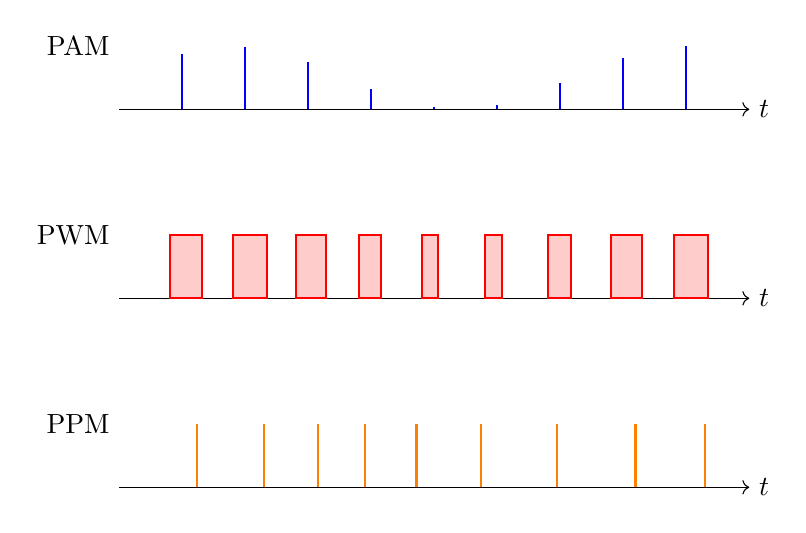
\begin{tikzpicture}[scale=0.8]
        % PAM
        \node [left] at (0, 7) {PAM};
        \draw [->] (0, 6) -- (10, 6) node[right] {$t$};
        \foreach \x in {1,2,3,4,5,6,7,8,9} {
            \pgfmathsetmacro{\yval}{6 + 0.5 + 0.5*sin(\x*50)}
            \draw [thick, blue] (\x, 6) -- (\x, \yval);
        }
        
        % PWM
        \node [left] at (0, 4) {PWM};
        \draw [->] (0, 3) -- (10, 3) node[right] {$t$};
        \foreach \x in {1,2,3,4,5,6,7,8,9} {
            \pgfmathsetmacro{\width}{0.2 + 0.15*sin(\x*50)}
            \draw [thick, red, fill=red!20] (\x-0.2, 3) rectangle (\x+\width, 4);
        }
            
        % PPM
        \node [left] at (0, 1) {PPM};
        \draw [->] (0, 0) -- (10, 0) node[right] {$t$};
        \foreach \x in {1,2,3,4,5,6,7,8,9} {
            \pgfmathsetmacro{\shift}{0.3*sin(\x*50)}
            \draw [thick, orange] (\x+\shift, 0) -- (\x+\shift, 1);
        }
    \end{tikzpicture}
    \end{center}

    \begin{mnemonicbox}
    "Amplitude varies height, Width varies length, Position varies timing"
    \end{mnemonicbox}
\end{solutionbox}

\questionmarks{2}{a}{3}
\textbf{Differentiate between bit, symbol and Baud rate.}

\begin{solutionbox}
    \textbf{Answer}:

    \begin{tabulary}{\textwidth}{|L|L|L|L|}
    \hline
    \textbf{Parameter} & \textbf{Bit} & \textbf{Symbol} & \textbf{Baud Rate} \\
    \hline
    \textbf{Definition} & Binary digit (0 or 1) & Group of bits & Number of symbols transmitted per second \\
    \hline
    \textbf{Unit} & No unit & No unit & Symbols per second (Baud) \\
    \hline
    \textbf{Relationship} & Basic unit of digital information & Multiple bits form one symbol & Baud rate $\times$ bits per symbol = bit rate \\
    \hline
    \textbf{Example} & 0, 1 & In 4-QAM, each symbol represents 2 bits & 1200 baud means 1200 symbols per second \\
    \hline
    \end{tabulary}

    \begin{mnemonicbox}
    "Bits Build Symbols, Bauds Show Speed"
    \end{mnemonicbox}
\end{solutionbox}

\questionmarks{2}{b}{4}
\textbf{State advantages and disadvantage of SSB over DSB.}

\begin{solutionbox}
    \textbf{Answer}:

    \begin{tabulary}{\textwidth}{|L|L|}
    \hline
    \textbf{Advantages of SSB over DSB} & \textbf{Disadvantages of SSB over DSB} \\
    \hline
    \textbf{Bandwidth}: Requires only half the bandwidth & \textbf{Circuit Complexity}: More complex modulation and demodulation \\
    \hline
    \textbf{Power Efficiency}: Transmits only one sideband, saving power & \textbf{Receiver Design}: Requires precise frequency synchronization \\
    \hline
    \textbf{Less Fading}: Reduced selective fading effects & \textbf{Low Frequency Loss}: May lose low frequency components \\
    \hline
    \textbf{Less Interference}: Reduced adjacent channel interference & \textbf{Cost}: More expensive implementation \\
    \hline
    \end{tabulary}

    \begin{mnemonicbox}
    "SSB Saves Bandwidth Power but Costs Complex Hardware"
    \end{mnemonicbox}
\end{solutionbox}

\questionmarks{2}{c}{7}
\textbf{Compare Amplitude Modulation (AM) and Frequency Modulation (FM).}

\begin{solutionbox}
    \textbf{Answer}:

    \begin{tabulary}{\textwidth}{|L|L|L|}
    \hline
    \textbf{Parameter} & \textbf{AM} & \textbf{FM} \\
    \hline
    \textbf{Modulated Parameter} & Amplitude of carrier & Frequency of carrier \\
    \hline
    \textbf{Bandwidth} & Narrow ($2 \times f_m$) & Wide ($2 \times (f_m + \Delta f)$) \\
    \hline
    \textbf{Noise Immunity} & Poor & Excellent \\
    \hline
    \textbf{Power Efficiency} & Poor (carrier contains most power) & Good \\
    \hline
    \textbf{Circuit Complexity} & Simple & Complex \\
    \hline
    \textbf{Quality} & Lower & Higher \\
    \hline
    \textbf{Applications} & Broadcasting (MW), Aircraft communication & FM radio, TV sound, Mobile communications \\
    \hline
    \end{tabulary}

    \textbf{Diagram:}

    \begin{center}
    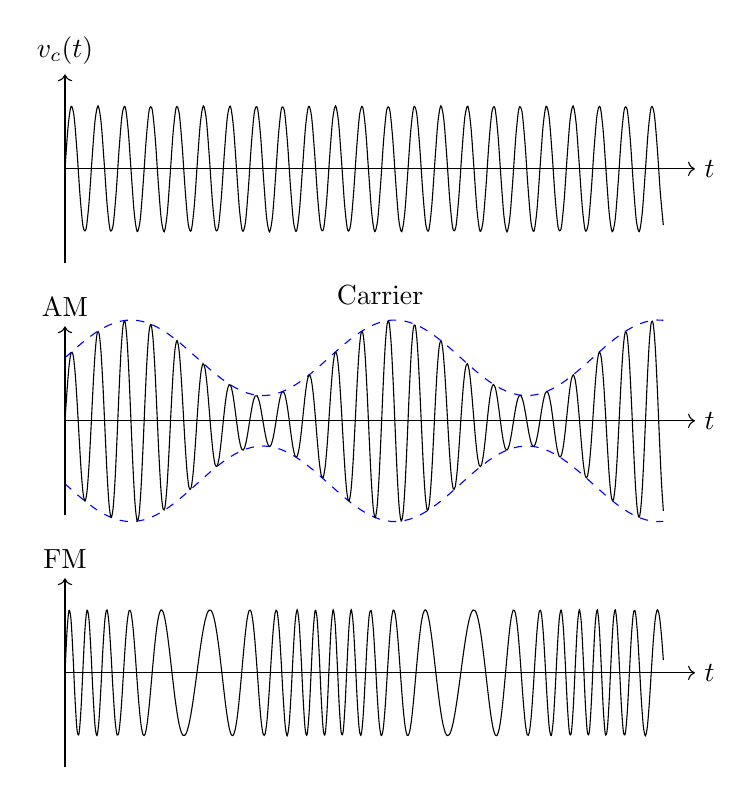
\begin{tikzpicture}[scale=0.8]
        % Carrier
        \begin{scope}[yshift=4cm]
            \draw[->] (0,0) -- (10,0) node[right] {$t$};
            \draw[->] (0,-1.5) -- (0,1.5) node[above] {$v_c(t)$};
            \draw[domain=0:9.5, samples=200, smooth] plot (\x, {1*sin(15*\x r)});
            \node at (5,-2) {Carrier};
        \end{scope}

        % AM
        \begin{scope}[yshift=0cm]
            \draw[->] (0,0) -- (10,0) node[right] {$t$};
            \draw[->] (0,-1.5) -- (0,1.5) node[above] {AM};
            % Envelope
            \draw[dashed, blue] plot[domain=0:9.5, samples=100] (\x, {1 + 0.6*sin(1.5*\x r)});
            \draw[dashed, blue] plot[domain=0:9.5, samples=100] (\x, {-(1 + 0.6*sin(1.5*\x r))});
            % Signal
            \draw[domain=0:9.5, samples=300, smooth] plot (\x, {(1 + 0.6*sin(1.5*\x r)) * sin(15*\x r)});
        \end{scope}

        % FM
        \begin{scope}[yshift=-4cm]
            \draw[->] (0,0) -- (10,0) node[right] {$t$};
            \draw[->] (0,-1.5) -- (0,1.5) node[above] {FM};
            \draw[domain=0:9.5, samples=300, smooth] plot (\x, {sin((15*\x + 5*sin(1.5*\x r)) r)});
        \end{scope}
    \end{tikzpicture}
    \end{center}

    \begin{mnemonicbox}
    "AM Alters strength, FM Fluctuates timing"
    \end{mnemonicbox}
\end{solutionbox}

\questionmarks{3}{a}{3}
\textbf{Compare AM receiver with FM receiver.}

\begin{solutionbox}
    \textbf{Answer}:

    \begin{tabulary}{\textwidth}{|L|L|L|}
    \hline
    \textbf{Parameter} & \textbf{AM Receiver} & \textbf{FM Receiver} \\
    \hline
    \textbf{IF Frequency} & 455 kHz & 10.7 MHz \\
    \hline
    \textbf{Detector} & Envelope detector & Discriminator/Ratio detector/PLL \\
    \hline
    \textbf{Bandwidth} & Narrow ($\pm$5 kHz) & Wide ($\pm$75 kHz) \\
    \hline
    \textbf{Special Circuits} & Simple & Limiter, De-emphasis \\
    \hline
    \textbf{Complexity} & Simple & Complex \\
    \hline
    \end{tabulary}

    \begin{mnemonicbox}
    "AM Accepts Minimal bandwidth; FM Features More circuits"
    \end{mnemonicbox}
\end{solutionbox}

\questionmarks{3}{b}{4}
\textbf{Define sampling? Explain types of sampling in brief.}

\begin{solutionbox}
    \textbf{Answer}:

    \textbf{Sampling}: Process of converting continuous-time signal into discrete-time signal by taking samples at regular intervals.

    \begin{tabulary}{\textwidth}{|L|L|L|}
    \hline
    \textbf{Type of Sampling} & \textbf{Description} & \textbf{Characteristics} \\
    \hline
    \textbf{Ideal Sampling} & Instantaneous samples of the signal & Perfect but theoretical, uses impulse function \\
    \hline
    \textbf{Natural Sampling} & Signal is sampled for short durations & Top of pulses follow original signal \\
    \hline
    \textbf{Flat-top Sampling} & Samples held constant until next sample & Creates staircase approximation, easier to implement \\
    \hline
    \end{tabulary}

    \textbf{Diagram:}

    \begin{center}
    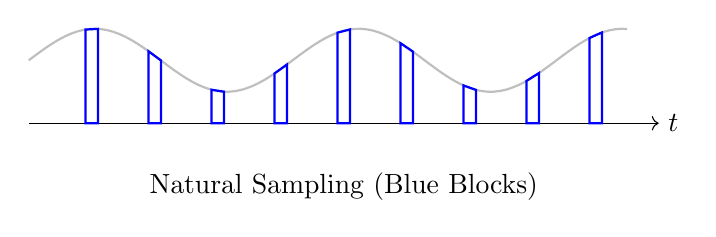
\begin{tikzpicture}[scale=0.8]
        \draw[->] (0,0) -- (10,0) node[right] {$t$};
        \draw[thick, gray, opacity=0.5] plot[domain=0:9.5, samples=100] (\x, {1 + 0.5*sin(1.5*\x r)});
        
        % Natural Sampling
        \foreach \x in {1,2,3,4,5,6,7,8,9} {
           \draw [thick, blue] (\x-0.1, 0) -- (\x-0.1, {1 + 0.5*sin(1.5*(\x-0.1) r)}) -- (\x+0.1, {1 + 0.5*sin(1.5*(\x+0.1) r)}) -- (\x+0.1, 0) -- cycle;
        }
        \node at (5,-1) {Natural Sampling (Blue Blocks)};
    \end{tikzpicture}
    \end{center}

    \begin{mnemonicbox}
    "Ideal takes Instants, Natural follows Nicely, Flat stays Fixed"
    \end{mnemonicbox}
\end{solutionbox}

\questionmarks{3}{c}{7}
\textbf{Draw and explain the block diagram of FM receiver. What is the use of Limiter in FM receiver?}

\begin{solutionbox}
    \textbf{Answer}:

    \begin{center}
    \begin{tikzpicture}[auto, node distance=2cm, >=latex]
        % Nodes
        \node [gtu block] (rf) {RF Amplifier};
        \node [left of=rf, node distance=2.5cm] (ant) {Antenna};
        \node [gtu block, right of=rf, node distance=3cm] (mixer) {Mixer};
        \node [gtu block, below of=mixer, node distance=2cm] (lo) {Local Oscillator};
        \node [gtu block, right of=mixer, node distance=2.5cm] (if) {IF Amplifier};
        \node [gtu block, right of=if, node distance=2.5cm] (lim) {Limiter};
        \node [gtu block, right of=lim, node distance=2.5cm] (disc) {Discriminator};
        \node [gtu block, below of=lim, node distance=2cm] (deemp) {De-emphasis};
        \node [gtu block, left of=deemp, node distance=3cm] (af) {AF Amplifier};
        \node [left of=af, node distance=2.5cm] (spk) {Speaker};

        % Connections
        \draw [gtu arrow] (ant) -- (rf);
        \draw [gtu arrow] (rf) -- (mixer);
        \draw [gtu arrow] (lo) -- (mixer);
        \draw [gtu arrow] (mixer) -- (if);
        \draw [gtu arrow] (if) -- (lim);
        \draw [gtu arrow] (lim) -- (disc);
        \draw [gtu arrow] (disc.south) -- ++(0,-0.5) -| (deemp.north);
        \draw [gtu arrow] (deemp) -- (af);
        \draw [gtu arrow] (af) -- (spk);

    \end{tikzpicture}
    \end{center}

    \begin{tabulary}{\textwidth}{|L|L|}
    \hline
    \textbf{Block} & \textbf{Function} \\
    \hline
    \textbf{RF Amplifier} & Amplifies weak RF signal and provides selectivity \\
    \hline
    \textbf{Mixer/Local Oscillator} & Converts RF to IF (10.7 MHz) \\
    \hline
    \textbf{IF Amplifier} & Provides gain and selectivity at fixed frequency \\
    \hline
    \textbf{Limiter} & Removes amplitude variations, preserves frequency variations \\
    \hline
    \textbf{Discriminator} & Converts frequency variations to amplitude variations \\
    \hline
    \textbf{De-emphasis} & Reduces high-frequency noise \\
    \hline
    \textbf{AF Amplifier} & Amplifies recovered audio for speaker \\
    \hline
    \end{tabulary}

    \textbf{Limiter Function}: Removes amplitude variations from the FM signal before demodulation to ensure noise immunity, as information in FM is contained in frequency variations, not amplitude.

    \begin{mnemonicbox}
    "Radio Mixers Increase Frequency; Limiters Discriminate Audio Sound"
    \end{mnemonicbox}
\end{solutionbox}

\questionmarks{3}{a}{3}
\textbf{Describe the concept of single side band (SSB) transmission.}

\begin{solutionbox}
    \textbf{Answer}:

    \textbf{Single Sideband (SSB) Transmission}: Technique where only one sideband (upper or lower) is transmitted while suppressing the carrier and other sideband.

    \begin{center}
    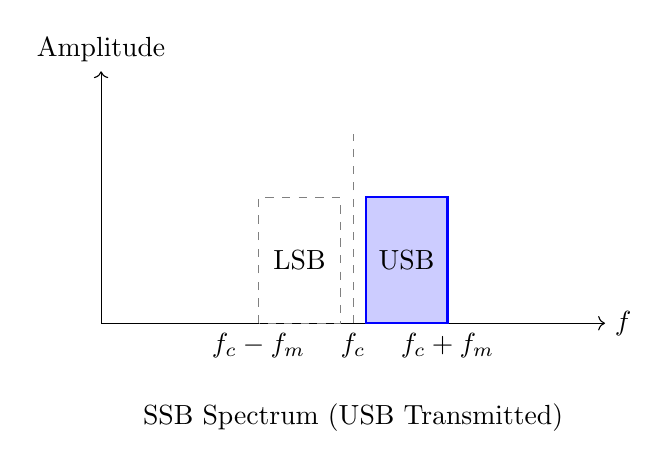
\begin{tikzpicture}[scale=0.8]
        \draw[->] (0,0) -- (8,0) node[right] {$f$};
        \draw[->] (0,0) -- (0,4) node[above] {Amplitude};
        
        % Carrier (Suppressed)
        \draw[dashed, gray] (4,0) -- (4,3);
        \node[below] at (4,0) {$f_c$};
        
        % LSB (Suppressed)
        \draw[dashed, gray] (2.5,0) rectangle (3.8, 2);
        \node at (3.15, 1) {LSB};
        \node[below] at (2.5,0) {$f_c-f_m$};
        
        % USB (Transmitted)
        \draw[thick, blue, fill=blue!20] (4.2,0) rectangle (5.5, 2);
        \node at (4.85, 1) {USB};
        \node[below] at (5.5,0) {$f_c+f_m$};
        
        \node at (4, -1.5) {SSB Spectrum (USB Transmitted)};
    \end{tikzpicture}
    \end{center}

    \begin{itemize}
        \item \textbf{Bandwidth}: Requires only half the bandwidth ($f_c \pm f_m$).
        \item \textbf{Power Efficiency}: More efficient as power concentrated in one sideband.
        \item \textbf{Types}: USB (Upper Sideband) and LSB (Lower Sideband).
    \end{itemize}

    \begin{mnemonicbox}
    "SSB Saves Spectrum Bandwidth"
    \end{mnemonicbox}
\end{solutionbox}

\questionmarks{3}{b}{4}
\textbf{Explain pre-emphasis \& de-emphasis circuit.}

\begin{solutionbox}
    \textbf{Answer}:

    \begin{tabulary}{\textwidth}{|L|L|L|}
    \hline
    \textbf{Parameter} & \textbf{Pre-emphasis} & \textbf{De-emphasis} \\
    \hline
    \textbf{Location} & Transmitter & Receiver \\
    \hline
    \textbf{Circuit Type} & High-pass RC network & Low-pass RC network \\
    \hline
    \textbf{Function} & Boosts high frequencies before transmission & Attenuates high frequencies after reception \\
    \hline
    \textbf{Purpose} & Improves SNR for high frequencies & Restores original frequency response \\
    \hline
    \end{tabulary}

    \textbf{Circuit Diagram:}

    \begin{center}
    \begin{circuitikz}[scale=0.8]
        % Pre-emphasis
        \draw (0,4) node[left] {Pre-emphasis} to[short, o-] (1,4); 
        \draw (1,4) to[R, l=$R$] (3,4);
        \draw (1,4) -- (1, 5.5) to[C, l=$C$] (3,5.5) -- (3,4);
        \draw (3,4) -- (4,4) to[R, l=$R_L$] (4,2) node[ground] {};
        \draw (3,4) to[short, -o] (5,4) node[right] {$V_{out}$};

        % De-emphasis
        \draw (7,4) node[left] {De-emphasis} to[short, o-] (8,4) to[R, l=$R$] (10,4) -- (11,4) to[short, -o] (12,4) node[right] {$V_{out}$};
        \draw (10,4) to[C, l=$C$] (10,2) node[ground] {};
    \end{circuitikz}
    \end{center}

    \begin{mnemonicbox}
    "Pre Pushes highs, De Drops them"
    \end{mnemonicbox}
\end{solutionbox}

\questionmarks{3}{c}{7}
\textbf{Illustrate generation of FM signal using Phase lock loop technique.}

\begin{solutionbox}
    \textbf{Answer}:

    \begin{center}
    \begin{tikzpicture}[auto, node distance=2.5cm, >=latex]
        \node [gtu block] (pd) {Phase Detector};
        \node [gtu block, right of=pd, node distance=3.5cm] (lf) {Loop Filter};
        \node [gtu block, right of=lf, node distance=3.5cm] (vco) {VCO};
        \node [gtu block, below of=pd, node distance=2cm] (ref) {Reference Oscillator};
        \node [above of=lf, node distance=1.5cm] (input) {Modulating Signal};

        \draw [gtu arrow] (ref) -- (pd);
        \draw [gtu arrow] (pd) -- (lf);
        \draw [gtu arrow] (lf) -- (vco);
        \draw [gtu arrow] (vco.south) -- ++(0,-1) -| (pd.south);
        \draw [gtu arrow] (vco.east) -- ++(1,0) node[right] {FM Output};
        \draw [gtu arrow] (input) -- (lf);
    \end{tikzpicture}
    \end{center}

    \begin{tabulary}{\textwidth}{|L|L|}
    \hline
    \textbf{Component} & \textbf{Function} \\
    \hline
    \textbf{Phase Detector} & Compares reference and VCO signals, generates error voltage \\
    \hline
    \textbf{Loop Filter} & Filters error voltage and combines with modulating signal \\
    \hline
    \textbf{VCO} & Generates frequency based on control voltage \\
    \hline
    \textbf{Reference Oscillator} & Provides stable reference frequency \\
    \hline
    \end{tabulary}

    \textbf{Working Process:}
    \begin{enumerate}
        \item Modulating signal is applied to loop filter.
        \item VCO frequency shifts proportional to modulating signal.
        \item Phase detector generates error signal.
        \item Loop maintains lock while allowing frequency modulation.
        \item Output of VCO is the FM signal.
    \end{enumerate}

    \begin{mnemonicbox}
    "Phase Locks, Voltage Controls, Frequency Modulates"
    \end{mnemonicbox}
\end{solutionbox}

\questionmarks{4}{a}{3}
\textbf{Explain quantization process and its importance.}

\begin{solutionbox}
    \textbf{Answer}:

    \textbf{Quantization}: Process of mapping continuous amplitude values to a finite set of discrete levels in analog-to-digital conversion.

    \begin{tabulary}{\textwidth}{|L|L|}
    \hline
    \textbf{Aspect} & \textbf{Description} \\
    \hline
    \textbf{Process} & Dividing amplitude range into fixed levels and assigning digital values \\
    \hline
    \textbf{Types} & Uniform (equal steps) and Non-uniform (variable steps) \\
    \hline
    \textbf{Error} & Difference between actual and quantized value (quantization noise) \\
    \hline
    \end{tabulary}

    \textbf{Importance}:
    \begin{itemize}
        \item Enables digital representation of analog signals.
        \item Determines resolution and accuracy of digital signal.
        \item Affects signal-to-noise ratio in digital systems.
    \end{itemize}

    \begin{mnemonicbox}
    "Quantization Creates Digital from Analog"
    \end{mnemonicbox}
\end{solutionbox}

\questionmarks{4}{b}{4}
\textbf{Explain different characteristics of Radio receiver.}

\begin{solutionbox}
    \textbf{Answer}:

    \begin{tabulary}{\textwidth}{|L|L|L|}
    \hline
    \textbf{Characteristic} & \textbf{Definition} & \textbf{Significance} \\
    \hline
    \textbf{Sensitivity} & Ability to receive weak signals & Determines reception range \\
    \hline
    \textbf{Selectivity} & Ability to separate adjacent channels & Prevents interference \\
    \hline
    \textbf{Fidelity} & Accuracy of reproduction & Determines sound quality \\
    \hline
    \textbf{Image Rejection} & Ability to reject image frequency & Prevents unwanted reception \\
    \hline
    \end{tabulary}

    \textbf{Diagram:}

    \begin{center}
    \begin{tikzpicture}[gtu tree]
    \node [gtu block] {Radio Receiver Characteristics}
        child {node [gtu state] {Sensitivity\\($\mu$V)}}
        child {node [gtu state] {Selectivity\\(Q factor)}}
        child {node [gtu state] {Fidelity\\(Freq resp)}}
        child {node [gtu state] {Image Rejection\\(Image ratio)}};
    \end{tikzpicture}
    \end{center}

    \begin{mnemonicbox}
    "Sensitive Selection Faithfully Images"
    \end{mnemonicbox}
\end{solutionbox}

\questionmarks{4}{c}{7}
\textbf{Draw and explain the block diagram of PCM transmitter and receiver.}

\begin{solutionbox}
    \textbf{Answer}:

    \textbf{PCM Transmitter:}
    \begin{center}
    \begin{tikzpicture}[auto, node distance=2.2cm, >=latex]
        \node [gtu block] (aa) {Anti-aliasing Filter};
        \node [left of=aa, node distance=2.5cm] (in) {Input};
        \node [gtu block, right of=aa] (sh) {S/H};
        \node [gtu block, right of=sh] (quant) {Quantizer};
        \node [gtu block, below of=quant, node distance=2cm] (enc) {Encoder};
        \node [gtu block, left of=enc] (lc) {Line Coder};
        \node [left of=lc, node distance=2.5cm] (out) {To Channel};

        \draw [gtu arrow] (in) -- (aa);
        \draw [gtu arrow] (aa) -- (sh);
        \draw [gtu arrow] (sh) -- (quant);
        \draw [gtu arrow] (quant) -- (enc);
        \draw [gtu arrow] (enc) -- (lc);
        \draw [gtu arrow] (lc) -- (out);
    \end{tikzpicture}
    \end{center}

    \textbf{PCM Receiver:}
    \begin{center}
    \begin{tikzpicture}[auto, node distance=2.2cm, >=latex]
        \node [gtu block] (ld) {Line Decoder};
        \node [left of=ld, node distance=2.5cm] (in) {From Channel};
        \node [gtu block, right of=ld] (reg) {Regenerator};
        \node [gtu block, right of=reg] (dec) {Decoder};
        \node [gtu block, below of=dec, node distance=2cm] (recon) {Reconstruction Filter};
        \node [left of=recon, node distance=3cm] (out) {Output};

        \draw [gtu arrow] (in) -- (ld);
        \draw [gtu arrow] (ld) -- (reg);
        \draw [gtu arrow] (reg) -- (dec);
        \draw [gtu arrow] (dec) -- (recon);
        \draw [gtu arrow] (recon) -- (out);
    \end{tikzpicture}
    \end{center}

    \begin{tabulary}{\textwidth}{|L|L|}
    \hline
    \textbf{Block} & \textbf{Function} \\
    \hline
    \textbf{Anti-aliasing Filter} & Limits input bandwidth to prevent aliasing \\
    \hline
    \textbf{Sample \& Hold} & Converts continuous signal to discrete-time samples \\
    \hline
    \textbf{Quantizer} & Converts sample amplitudes to discrete levels \\
    \hline
    \textbf{Encoder} & Converts quantized values to binary code \\
    \hline
    \textbf{Line Coder} & Formats binary data for transmission \\
    \hline
    \textbf{Decoder} & Converts binary code back to quantized values \\
    \hline
    \textbf{Reconstruction Filter} & Smooths the stepped output to recover original signal \\
    \hline
    \end{tabulary}

    \begin{mnemonicbox}
    "Sample, Quantize, Encode, Transmit; Decode, Reconstruct, Output"
    \end{mnemonicbox}
\end{solutionbox}

\questionmarks{4}{a}{3}
\textbf{Compare Natural and Flat top sampling.}

\begin{solutionbox}
    \textbf{Answer}:

    \begin{tabulary}{\textwidth}{|L|L|L|}
    \hline
    \textbf{Parameter} & \textbf{Natural Sampling} & \textbf{Flat-top Sampling} \\
    \hline
    \textbf{Shape} & Top of pulses follow input signal & Constant amplitude during sampling interval \\
    \hline
    \textbf{Implementation} & More difficult (analog switch) & Easier (sample and hold circuit) \\
    \hline
    \textbf{Spectrum} & Less harmonics & More harmonics \\
    \hline
    \textbf{Reconstruction} & Easier, more accurate & Requires compensation for distortion \\
    \hline
    \end{tabulary}

    \textbf{Diagram:}

    \begin{center}
    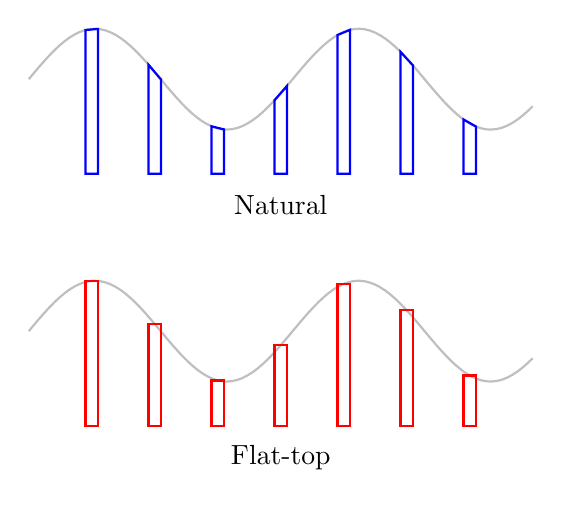
\begin{tikzpicture}[scale=0.8]
        \draw[thick, gray, opacity=0.5] plot[domain=0:8, samples=100] (\x, {1.5 + 0.8*sin(\x*1.5 r)});
        
        % Natural
        \foreach \x in {1,2,3,4,5,6,7} {
            \draw[thick, blue] (\x-0.1, 0) -- (\x-0.1, {1.5 + 0.8*sin((\x-0.1)*1.5 r)}) 
                -- (\x+0.1, {1.5 + 0.8*sin((\x+0.1)*1.5 r)}) -- (\x+0.1, 0) -- cycle;
        }
        \node at (4, -0.5) {Natural};

        % Flat-top
        \begin{scope}[yshift=-4cm]
            \draw[thick, gray, opacity=0.5] plot[domain=0:8, samples=100] (\x, {1.5 + 0.8*sin(\x*1.5 r)});
            \foreach \x in {1,2,3,4,5,6,7} {
                \draw[thick, red] (\x-0.1, 0) -- (\x-0.1, {1.5 + 0.8*sin(\x*1.5 r)}) 
                    -- (\x+0.1, {1.5 + 0.8*sin(\x*1.5 r)}) -- (\x+0.1, 0) -- cycle;
            }
            \node at (4, -0.5) {Flat-top};
        \end{scope}
    \end{tikzpicture}
    \end{center}

    \begin{mnemonicbox}
    "Natural Follows, Flat Freezes"
    \end{mnemonicbox}
\end{solutionbox}

\questionmarks{4}{b}{4}
\textbf{Explain Diode Detector circuit.}

\begin{solutionbox}
    \textbf{Answer}:

    \textbf{Diode Detector Circuit}: Used for demodulation of AM signals by extracting the envelope of the modulated wave.

    \begin{center}
    \begin{circuitikz}[scale=0.9]
        \draw (0,2) to[short, o-] (1,2) to[D, l=$D$] (3,2);
        \draw (3,2) -- (4,2) to[C, l=$C$] (4,0) node[ground] {};
        \draw (3,2) -- (6,2) to[R, l=$R$] (6,0) node[ground] {};
        \draw (6,2) to[short, -o] (7,2) node[right] {Output};
        \draw (0,0) node[ground] {} to[short, o-] (1,0);
        \node at (-0.5, 1) {Input AM};
    \end{circuitikz}
    \end{center}

    \begin{tabulary}{\textwidth}{|L|L|}
    \hline
    \textbf{Component} & \textbf{Function} \\
    \hline
    \textbf{Diode (D)} & Rectifies the AM signal, passes only positive half \\
    \hline
    \textbf{Capacitor (C)} & Charges to peak value, smooths out carrier \\
    \hline
    \textbf{Resistor (R)} & Controls discharge time of capacitor \\
    \hline
    \end{tabulary}

    \textbf{Working}:
    \begin{enumerate}
        \item Diode rectifies AM signal.
        \item Capacitor charges to peak value.
        \item RC time constant allows capacitor to follow envelope.
        \item Output follows the original modulating signal.
    \end{enumerate}

    \begin{mnemonicbox}
    "Diode Detects, Capacitor Captures"
    \end{mnemonicbox}
\end{solutionbox}

\questionmarks{4}{c}{7}
\textbf{Draw and explain the block diagram of Delta Modulation.}

\begin{solutionbox}
    \textbf{Answer}:

    \textbf{Delta Modulation Transmitter:}
    \begin{center}
    \begin{tikzpicture}[auto, node distance=2.5cm, >=latex]
        \node [gtu block] (comp) {Comparator};
        \node [left of=comp, node distance=2.5cm] (in) {Input};
        \node [gtu block, right of=comp] (quant) {1-bit Quant};
        \node [gtu block, below of=comp, node distance=2cm] (integ) {Integrator};
        \node [right of=quant, node distance=2.5cm] (out) {To Channel};

        \draw [gtu arrow] (in) -- (comp);
        \draw [gtu arrow] (comp) -- (quant);
        \draw [gtu arrow] (quant) -- (out);
        \draw [gtu arrow] (quant.south) |- (integ.east);
        \draw [gtu arrow] (integ) -- (comp);
    \end{tikzpicture}
    \end{center}

    \textbf{Delta Modulation Receiver:}
    \begin{center}
    \begin{tikzpicture}[auto, node distance=2.5cm, >=latex]
        \node [gtu block] (integ) {Integrator};
        \node [left of=integ, node distance=2.5cm] (in) {Input};
        \node [gtu block, right of=integ] (lpf) {LPF};
        \node [right of=lpf, node distance=2.5cm] (out) {Output};

        \draw [gtu arrow] (in) -- (integ);
        \draw [gtu arrow] (integ) -- (lpf);
        \draw [gtu arrow] (lpf) -- (out);
    \end{tikzpicture}
    \end{center}

    \begin{tabulary}{\textwidth}{|L|L|}
    \hline
    \textbf{Component} & \textbf{Function} \\
    \hline
    \textbf{Comparator} & Compares input with predicted value \\
    \hline
    \textbf{1-bit Quantizer} & Outputs binary 1 if input $>$ predicted, 0 if input $<$ predicted \\
    \hline
    \textbf{Integrator} & Generates predicted value by integrating previous output \\
    \hline
    \textbf{Low-pass Filter} & Smooths stepped output to recover original signal \\
    \hline
    \end{tabulary}

    \textbf{Limitations}:
    \begin{itemize}
        \item \textbf{Slope Overload}: Occurs when signal changes faster than step size can track.
        \item \textbf{Granular Noise}: Occurs during idle or constant parts of signal.
    \end{itemize}

    \begin{mnemonicbox}
    "Delta Detects Differences, Integrator Increments"
    \end{mnemonicbox}
\end{solutionbox}

\questionmarks{5}{a}{3}
\textbf{Illustrate working of DPCM.}

\begin{solutionbox}
    \textbf{Answer}:

    \textbf{DPCM (Differential Pulse Code Modulation)}: Encodes the difference between current sample and predicted value.

    \begin{center}
    \begin{tikzpicture}[auto, node distance=2.5cm, >=latex]
        \node [gtu block] (add) {Diff Gen};
        \node [left of=add, node distance=2cm] (in) {Input};
        \node [gtu block, right of=add] (quant) {Quantizer};
        \node [gtu block, right of=quant] (enc) {Encoder};
        \node [right of=enc, node distance=2cm] (out) {Tx};
        \node [gtu block, below of=quant, node distance=2cm] (invq) {Inv Quant};
        \node [gtu block, left of=invq] (pred) {Predictor};

        \draw [gtu arrow] (in) -- (add);
        \draw [gtu arrow] (add) -- (quant);
        \draw [gtu arrow] (quant) -- (enc);
        \draw [gtu arrow] (enc) -- (out);
        \draw [gtu arrow] (quant.south) -- (invq.north);
        \draw [gtu arrow] (invq) -- (pred);
        \draw [gtu arrow] (pred) -- (add);
    \end{tikzpicture}
    \end{center}

    \begin{itemize}
        \item \textbf{Predictor}: Estimates current sample based on previous samples.
        \item \textbf{Difference}: Only difference between actual and predicted is encoded.
        \item \textbf{Advantage}: Reduces bit rate compared to PCM by exploiting signal correlation.
    \end{itemize}

    \begin{mnemonicbox}
    "Differences Predicted Create Minimized bits"
    \end{mnemonicbox}
\end{solutionbox}

\questionmarks{5}{b}{4}
\textbf{Illustrate Adaptive Delta Modulation.}

\begin{solutionbox}
    \textbf{Answer}:

    \textbf{Adaptive Delta Modulation (ADM)}: Improved version of DM that varies step size based on signal characteristics.

    \begin{center}
    \begin{tikzpicture}[auto, node distance=2.2cm, >=latex]
        \node [gtu block] (comp) {Comparator};
        \node [left of=comp, node distance=2cm] (in) {Input};
        \node [gtu block, right of=comp] (pulse) {Pulse Gen};
        \node [gtu block, below of=pulse, node distance=1.5cm] (logic) {Step Logic};
        \node [gtu block, left of=logic] (integ) {Integrator};
        \node [right of=pulse, node distance=2cm] (out) {Tx};

        \draw [gtu arrow] (in) -- (comp);
        \draw [gtu arrow] (comp) -- (pulse);
        \draw [gtu arrow] (pulse) -- (out);
        \draw [gtu arrow] (pulse.south) -- (logic.north);
        \draw [gtu arrow] (logic) -- (integ);
        \draw [gtu arrow] (integ) -- (comp);
    \end{tikzpicture}
    \end{center}

    \textbf{Operation}:
    \begin{enumerate}
        \item If multiple 1's detected: increase step size to avoid slope overload.
        \item If multiple 0's detected: increase step size to track falling signal.
        \item If alternating 1's and 0's: decrease step size to reduce granular noise.
    \end{enumerate}

    \begin{mnemonicbox}
    "Adapting Delta Makes Slopes Trackable"
    \end{mnemonicbox}
\end{solutionbox}

\questionmarks{5}{c}{7}
\textbf{Illustrate TDM frame.}

\begin{solutionbox}
    \textbf{Answer}:

    \textbf{TDM (Time Division Multiplexing) Frame}: Structure used to combine multiple signals by assigning time slots.

    \textbf{Frame Structure:}
    \begin{center}
    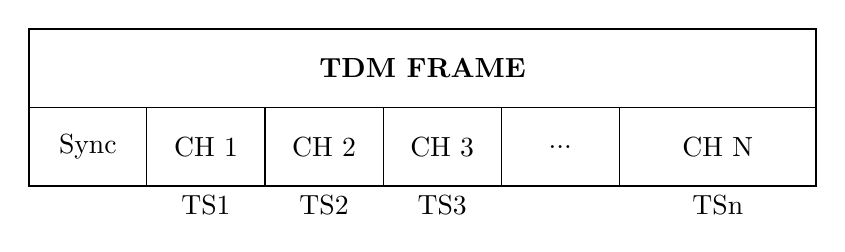
\begin{tikzpicture}
        \draw[thick] (0,0) rectangle (10, 2);
        \node at (5, 1.5) {\textbf{TDM FRAME}};
        
        \draw (0,0) rectangle (1.5, 1); \node at (0.75, 0.5) {Sync};
        \draw (1.5,0) rectangle (3, 1); \node at (2.25, 0.5) {CH 1};
        \draw (3,0) rectangle (4.5, 1); \node at (3.75, 0.5) {CH 2};
        \draw (4.5,0) rectangle (6, 1); \node at (5.25, 0.5) {CH 3};
        \draw (6,0) rectangle (7.5, 1); \node at (6.75, 0.5) {...};
        \draw (7.5,0) rectangle (10, 1); \node at (8.75, 0.5) {CH N};
        
        \node[below] at (2.25, 0) {TS1};
        \node[below] at (3.75, 0) {TS2};
        \node[below] at (5.25, 0) {TS3};
        \node[below] at (8.75, 0) {TSn};
    \end{tikzpicture}
    \end{center}

    \begin{tabulary}{\textwidth}{|L|L|}
    \hline
    \textbf{Component} & \textbf{Description} \\
    \hline
    \textbf{Frame Sync} & Pattern to identify frame boundaries \\
    \hline
    \textbf{Channel Sample} & Data from individual channel \\
    \hline
    \textbf{Time Slot (TS)} & Dedicated period for each channel \\
    \hline
    \textbf{Frame Duration} & Inversely proportional to sampling rate \\
    \hline
    \end{tabulary}

    \textbf{TDM Hierarchy:}
    \begin{itemize}
        \item Primary: 2.048 Mbps
        \item Secondary: 8.448 Mbps
        \item Tertiary: 34.368 Mbps
        \item Quaternary: 139.264 Mbps
    \end{itemize}

    \begin{mnemonicbox}
    "Frames Synchronize Time Slots During Multiplexing"
    \end{mnemonicbox}
\end{solutionbox}

\questionmarks{5}{a}{3}
\textbf{State difference between DM and ADM.}

\begin{solutionbox}
    \textbf{Answer}:

    \begin{tabulary}{\textwidth}{|L|L|L|}
    \hline
    \textbf{Parameter} & \textbf{Delta Modulation (DM)} & \textbf{Adaptive Delta Modulation (ADM)} \\
    \hline
    \textbf{Step Size} & Fixed step size & Variable step size \\
    \hline
    \textbf{Slope Overload} & Common problem & Reduced by adaptive step size \\
    \hline
    \textbf{Granular Noise} & High during slow variations & Reduced by adaptive step size \\
    \hline
    \textbf{Circuit Complexity} & Simpler & More complex \\
    \hline
    \textbf{Signal Quality} & Lower & Higher \\
    \hline
    \end{tabulary}

    \begin{mnemonicbox}
    "DM's Fixed Steps; ADM Adapts"
    \end{mnemonicbox}
\end{solutionbox}

\questionmarks{5}{b}{4}
\textbf{Explain the need of line coding. Explain AMI technique.}

\begin{solutionbox}
    \textbf{Answer}:

    \textbf{Need for Line Coding:}
    \begin{itemize}
        \item \textbf{DC Component}: To eliminate DC component for AC-coupled systems.
        \item \textbf{Synchronization}: To provide timing information for clock recovery.
        \item \textbf{Error Detection}: To enable detection of transmission errors.
        \item \textbf{Spectral Efficiency}: To shape signal spectrum for efficient bandwidth use.
        \item \textbf{Noise Immunity}: To provide resistance against channel noise.
    \end{itemize}

    \textbf{AMI (Alternate Mark Inversion) Technique:}

    \begin{tabulary}{\textwidth}{|L|L|}
    \hline
    \textbf{Parameter} & \textbf{Description} \\
    \hline
    \textbf{Encoding Rule} & Binary 0 $\rightarrow$ 0V, Binary 1 $\rightarrow$ Alternating +V/-V \\
    \hline
    \textbf{DC Component} & No DC component (balanced code) \\
    \hline
    \textbf{Error Detection} & Can detect violations in alternating pattern \\
    \hline
    \textbf{Bandwidth} & Requires less bandwidth than NRZ codes \\
    \hline
    \end{tabulary}

    \textbf{Diagram:}
    \begin{center}
    \begin{tikzpicture}[scale=0.8]
        \node [left] at (0, 1) {AMI};
        \draw [->] (0, 0) -- (12, 0) node[right] {$t$};
        \node at (0.5, 2) {1}; \node at (1.5, 2) {0}; \node at (2.5, 2) {1}; \node at (3.5, 2) {1}; 
        \node at (4.5, 2) {0}; \node at (5.5, 2) {0}; \node at (6.5, 2) {1}; \node at (7.5, 2) {0};
        
        % 1 0 1 1 0 0 1 0 (Alternating)
        \draw [thick, blue] (0,0) -- (0,1) -- (1,1) -- (1,0) -- (2,0) -- (2,-1) -- (3,-1) -- (3,0) -- (3,1) -- (4,1) -- (4,0) -- (6,0) -- (6,-1) -- (7,-1) -- (7,0) -- (8,0);
        
    \end{tikzpicture}
    \end{center}

    \begin{mnemonicbox}
    "Alternating Marks Invert Polarity"
    \end{mnemonicbox}
\end{solutionbox}

\questionmarks{5}{c}{7}
\textbf{Draw and explain block diagram of basic PCM-TDM system.}

\begin{solutionbox}
    \textbf{Answer}:

    \textbf{PCM-TDM Transmitter:}
    \begin{center}
    \begin{tikzpicture}[auto, node distance=2cm, >=latex]
        % Channels
        \node (ch1) {CH 1};
        \node [below of=ch1] (ch2) {CH 2};
        \node [below of=ch2] (ch3) {CH 3};
        
        % LPFs
        \node [gtu block, right of=ch1, node distance=2cm] (lpf1) {LPF};
        \node [gtu block, right of=ch2, node distance=2cm] (lpf2) {LPF};
        \node [gtu block, right of=ch3, node distance=2cm] (lpf3) {LPF};
        
        % Multiplexer (simplified as switch inputs)
        \node [gtu block, right of=lpf2, node distance=3cm, minimum height=3cm] (mux) {Mux};
        
        % PCM part
        \node [gtu block, right of=mux, node distance=2.5cm] (adc) {ADC/Enc};
        \node [gtu block, right of=adc] (lc) {Line Coder};
        \node [right of=lc] (out) {Tx};

        \draw [gtu arrow] (ch1) -- (lpf1);
        \draw [gtu arrow] (ch2) -- (lpf2);
        \draw [gtu arrow] (ch3) -- (lpf3);
        
        \draw [gtu arrow] (lpf1) -- (mux.160);
        \draw [gtu arrow] (lpf2) -- (mux.180);
        \draw [gtu arrow] (lpf3) -- (mux.200);
        
        \draw [gtu arrow] (mux) -- (adc);
        \draw [gtu arrow] (adc) -- (lc);
        \draw [gtu arrow] (lc) -- (out);
    \end{tikzpicture}
    \end{center}

    \begin{tabulary}{\textwidth}{|L|L|}
    \hline
    \textbf{Block} & \textbf{Function} \\
    \hline
    \textbf{Low-pass Filter} & Limits bandwidth to satisfy sampling theorem \\
    \hline
    \textbf{Multiplexer} & Sample \& Holds inputs and combines them sequentially \\
    \hline
    \textbf{ADC/Encoder} & Quantizes and encodes the multiplexed stream \\
    \hline
    \textbf{Line Coder} & Formats binary data for transmission \\
    \hline
    \textbf{Receiver} & Performs reverse operation (Decoder $\rightarrow$ Demux $\rightarrow$ LPFs) \\
    \hline
    \end{tabulary}

    \begin{mnemonicbox}
    "Multiple Channels Sample, Quantize, Encode; Decode, Demultiplex, Filter"
    \end{mnemonicbox}
\end{solutionbox}

\end{document}

